\documentclass[11pt,a4paper]{article}

\usepackage[utf8]{inputenc}
\usepackage[T1]{fontenc}
\usepackage[indonesian]{babel}
\usepackage[a4paper,margin=2.2cm]{geometry}
\usepackage{amsmath,amssymb,mathtools}
\usepackage{array,booktabs,longtable,tabularx,multirow}
\usepackage{enumitem}
\usepackage{graphicx}
\usepackage{float}
\usepackage{xcolor}
\usepackage{hyperref}
\usepackage{mdframed}
\usepackage{fancyhdr}
\usepackage{lastpage}
\usepackage{setspace}
\usepackage{titlesec}
\usepackage{ragged2e}

\hypersetup{colorlinks=false,pdfborder={0 0 0}}
\setlength{\parindent}{0pt}
\setlength{\parskip}{0.45em}
\renewcommand{\arraystretch}{1.2}
\setlist[itemize]{leftmargin=1.4em,itemsep=0.15em,topsep=0.2em}
\setlist[enumerate]{leftmargin=1.5em,itemsep=0.2em,topsep=0.2em}
\newcolumntype{Y}{>{\RaggedRight\arraybackslash}X}
\newcolumntype{C}[1]{>{\centering\arraybackslash}p{#1}}
\newcolumntype{L}[1]{>{\RaggedRight\arraybackslash}p{#1}}

\pagestyle{fancy}
\fancyhf{}
\lhead{MA25-31017 -- Pemodelan Komputasi dan Analisis Numerik}
\rhead{Tugas Besar 2026/2027}
\cfoot{\thepage\,/\pageref{LastPage}}
\setlength{\headheight}{14pt}

\titleformat{\section}{\large\bfseries}{\thesection.}{0.5em}{}
\titleformat{\subsection}{\normalsize\bfseries}{\thesubsection.}{0.5em}{}

\begin{document}
\small

% ==========================================================
% HEADER
% ==========================================================
\begin{center}
\begin{tabularx}{\textwidth}{L{2.4cm} Y}
\multirow{5}{*}{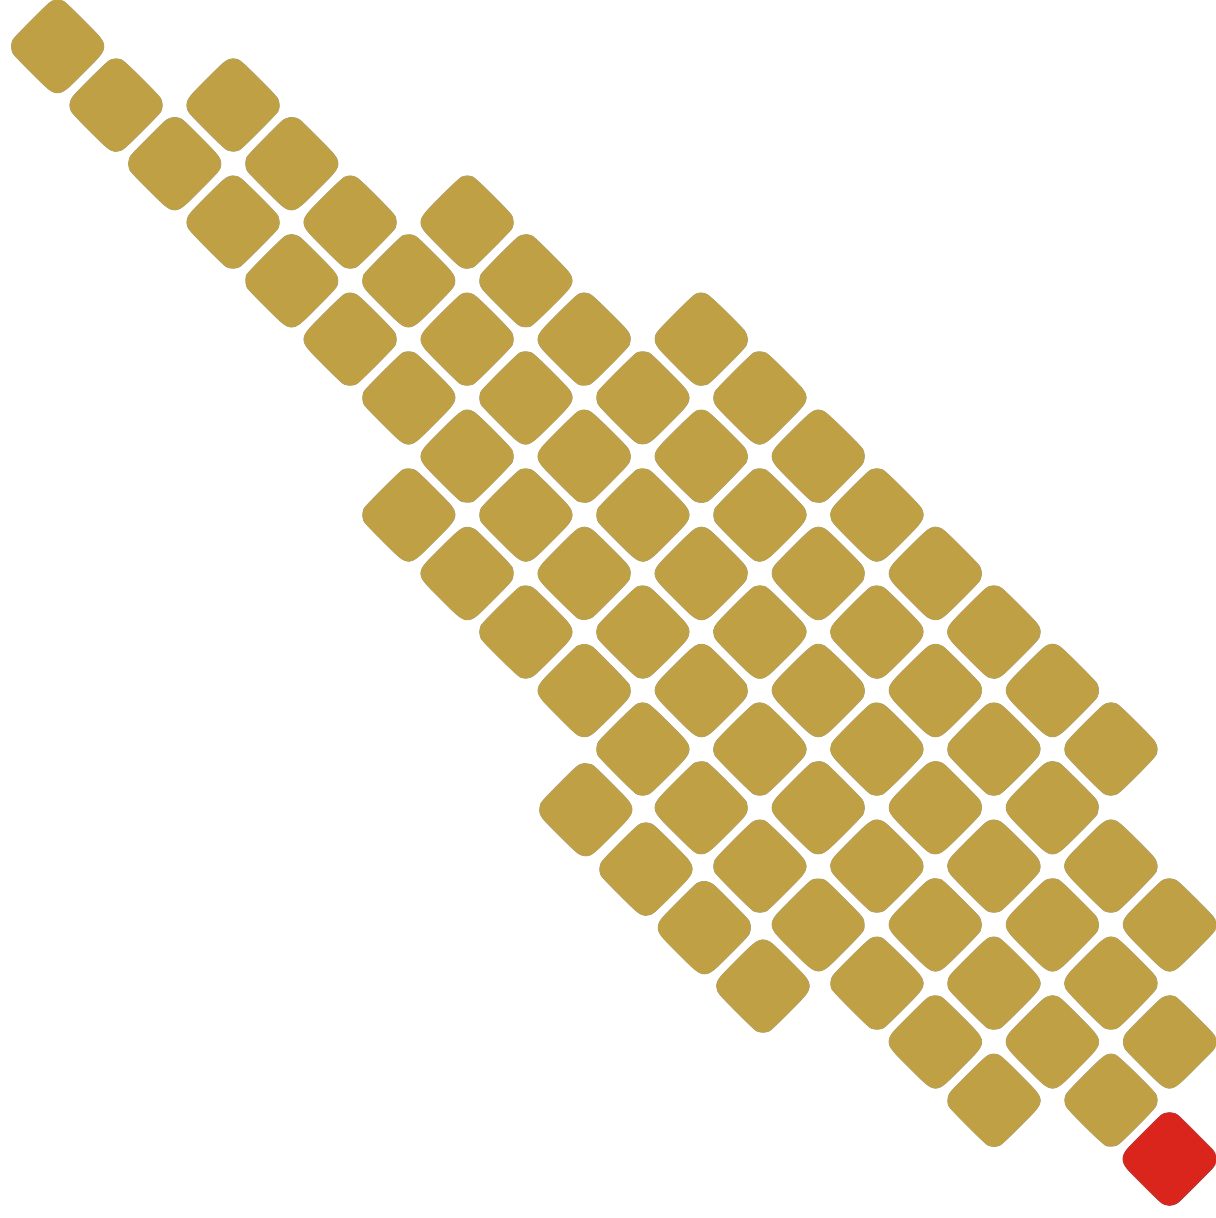
\includegraphics[width=2.1cm]{logo-itera-baru.png}}
& \textbf{Institut Teknologi Sumatera -- Fakultas Sains} \\
& \textbf{Program Studi Matematika} \\
& Semester Ganjil Tahun Akademik 2026/2027 \\
& Kode/Mata Kuliah: \textbf{MA25-31017 / Pemodelan Komputasi dan Analisis Numerik} \\
& Bentuk Pembelajaran: \textbf{Project-Based Learning, AI-Assisted} \\
\end{tabularx}
\end{center}

\vspace{0.4em}
\hrule
\vspace{0.8em}

\begin{center}
{\LARGE\bfseries PEDOMAN TUGAS BESAR}\\[0.25em]
{\large\bfseries AI-Assisted Computational Modeling Project}
\end{center}

\begin{mdframed}
\textbf{Gagasan utama.} Mahasiswa menyelesaikan satu masalah berbasis data ilmiah dengan membangun alur yang utuh: memahami masalah, memilih model, mengestimasi parameter, menjalankan prosedur numerik, memvalidasi hasil, menafsirkan dampaknya, dan menuliskannya sebagai artikel ilmiah. Metode numerik diposisikan sebagai \textbf{alat untuk menjawab masalah}, bukan sebagai tujuan akhir penelitian.
\end{mdframed}

% ==========================================================
\section{Tujuan dan Capaian yang Diukur}

Tugas besar dirancang untuk memberikan bekal riset komputasi yang dekat dengan praktik ilmiah: mencari literatur, menggunakan data nyata, menulis kode yang dapat direproduksi, menilai kualitas model, melakukan validasi numerik, menanggapi review, serta menggunakan AI secara kritis dan bertanggung jawab.

Mata kuliah MA25-31017 memetakan project ini terutama pada tiga CPL berikut.

\begin{longtable}{L{1.2cm} L{6.6cm} L{6.6cm}}
\toprule
\textbf{CPL} & \textbf{Makna dalam project} & \textbf{Bukti yang dinilai} \\
\midrule
\endfirsthead
\toprule
\textbf{CPL} & \textbf{Makna dalam project} & \textbf{Bukti yang dinilai} \\
\midrule
\endhead
CPL-6 & Menerapkan metode matematis/numerik dengan teknologi terkini, memperoleh solusi, lalu menginterpretasikan dan mengevaluasi solusi. & Implementasi SPL, estimasi parameter, akar, turunan, integral, ODE; residual, galat, konvergensi, benchmark, dan penjelasan algoritma. \\
CPL-7 & Menerapkan dan menganalisis model matematika untuk memecahkan masalah nyata serta mengevaluasi keakuratan, keterbatasan, dan relevansi model. & Pemilihan masalah, model, hubungan antarprosedur, interpretasi fenomena, pembahasan, keterbatasan, dan implikasi. \\
CPL-10 & Berpikir kritis, bekerja mandiri/tim, serta beradaptasi dengan perkembangan ilmu pengetahuan dan teknologi. & Literatur terverifikasi, reproducibility, provenance data/angka, pembagian kontribusi, response to reviewer, penggunaan AI, dan ujian individual. \\
\bottomrule
\end{longtable}

% ==========================================================
\section{Gambaran Project}

Setiap kelompok menggunakan \textbf{satu kasus/data utama}. Keenam komponen numerik berikut wajib dikerjakan dalam satu studi yang koheren:

\begin{enumerate}
    \item Sistem Persamaan Linear (SPL);
    \item pencarian akar persamaan;
    \item estimasi parameter;
    \item turunan numerik;
    \item integral numerik; dan
    \item penyelesaian Persamaan Diferensial Biasa (PDB/ODE).
\end{enumerate}

Keenam komponen tersebut \textbf{tidak boleh menjadi enam soal terpisah}. Mahasiswa harus menjelaskan mengapa suatu kuantitas perlu dihitung dan apa artinya bagi masalah yang sedang dikaji.

Contoh pertanyaan yang diharapkan:
\begin{itemize}
    \item kapan sistem mencapai kondisi kritis atau ambang tertentu;
    \item bagaimana laju fenomena berubah;
    \item berapa besar kuantitas yang terakumulasi selama suatu periode;
    \item parameter apa yang paling menjelaskan data;
    \item bagaimana perilaku model pada jangka waktu tertentu;
    \item apakah model cukup baik menjelaskan data;
    \item bagian mana dari perbedaan model-data yang berasal dari error numerik dan bagian mana yang berasal dari keterbatasan model.
\end{itemize}

\subsection*{Aturan Pemilihan Masalah dan Model untuk RA--RB}

Pemilihan dilakukan dari \textbf{masalah terlebih dahulu}, baru kemudian model yang kompatibel. Aturan kelas dibuat agar pilihan antarkelompok tidak identik tetapi tingkat pekerjaan tetap sebanding.

\begin{mdframed}
\begin{enumerate}
    \item Satu masalah hanya dapat dipilih oleh \textbf{satu kelompok di RA} dan \textbf{satu kelompok di RB}.
    \item Masalah yang sama boleh muncul sekali di RA dan sekali di RB, tetapi \textbf{modelnya wajib berbeda}.
    \item Pasangan \textbf{masalah + model} tidak boleh sama pada dua kelompok mana pun.
    \item Satu model dapat digunakan pada beberapa masalah yang berbeda apabila bentuk model dan interpretasinya relevan.
    \item Data utama dikunci berdasarkan masalah. File siap pakai disediakan di repository agar mahasiswa dapat langsung memulai eksplorasi dan pemodelan.
\end{enumerate}
\end{mdframed}


% ==========================================================
\section{Masalah dan Data Siap Pakai}

Project dimulai dari \textbf{masalah}, bukan dari nama metode atau nama model. Setiap kelompok membaca konteks masalah dan data terlebih dahulu, kemudian memilih salah satu model yang kompatibel. Model yang sama dapat digunakan pada beberapa masalah berbeda selama interpretasinya relevan.

Semua file berikut merupakan \textbf{data siap pakai} dan disimpan pada folder:
\begin{center}
\url{https://github.com/fauzirifky/Pemodelan-Komputasi-dan-Analisis-Numerik/tree/main/Tugas_Besar/data}
\end{center}

Mahasiswa dapat langsung mengunduh CSV dari tabel. File siap pakai bukan data sintetis. Beberapa merupakan subset atau transformasi terukur dari dataset publik; provenance lengkap disediakan pada \texttt{DATA\_SOURCES.md}.

\begin{longtable}{L{0.7cm} L{4.0cm} L{2.0cm} L{7.2cm}}
\toprule
\textbf{ID} & \textbf{Masalah} & \textbf{Data} & \textbf{Model yang dapat dipilih} \\
\midrule
\endfirsthead
\toprule
\textbf{ID} & \textbf{Masalah} & \textbf{Data} & \textbf{Model yang dapat dipilih} \\
\midrule
\endhead
P01 & Pertumbuhan bobot sapi Brahman & \href{https://raw.githubusercontent.com/fauzirifky/Pemodelan-Komputasi-dan-Analisis-Numerik/main/Tugas_Besar/data/P01_brahman_cattle.csv}{\textbf{Unduh CSV}} & Brody; von Bertalanffy; Gompertz growth \\
P02 & Pertumbuhan tumor & \href{https://raw.githubusercontent.com/fauzirifky/Pemodelan-Komputasi-dan-Analisis-Numerik/main/Tugas_Besar/data/P02_tumor_growth.csv}{\textbf{Unduh CSV}} & Logistic growth; Gompertz growth; von Bertalanffy-type \\
P03 & Farmakokinetik Theophylline oral & \href{https://raw.githubusercontent.com/fauzirifky/Pemodelan-Komputasi-dan-Analisis-Numerik/main/Tugas_Besar/data/P03_theophylline.csv}{\textbf{Unduh CSV}} & Bateman; Bateman + lag time; Mono-exponential \\
P04 & Farmakokinetik Indomethacin IV & \href{https://raw.githubusercontent.com/fauzirifky/Pemodelan-Komputasi-dan-Analisis-Numerik/main/Tugas_Besar/data/P04_indomethacin.csv}{\textbf{Unduh CSV}} & Mono-exponential; Bi-exponential; Two-stage bi-exponential \\
P05 & Degradasi kapasitas baterai NASA B0005 & \href{https://raw.githubusercontent.com/fauzirifky/Pemodelan-Komputasi-dan-Analisis-Numerik/main/Tugas_Besar/data/P05_nasa_b0005.csv}{\textbf{Unduh CSV}} & Linear degradation; Quadratic degradation; Offset exponential decay \\
P06 & Wabah influenza boarding school 1978 & \href{https://raw.githubusercontent.com/fauzirifky/Pemodelan-Komputasi-dan-Analisis-Numerik/main/Tugas_Besar/data/P06_influenza_boarding_school.csv}{\textbf{Unduh CSV}} & Gaussian epidemic curve; Gamma-shaped epidemic curve; SIR \\
P07 & Pertumbuhan ikan karang Acanthurus achilles & \href{https://raw.githubusercontent.com/fauzirifky/Pemodelan-Komputasi-dan-Analisis-Numerik/main/Tugas_Besar/data/P07_coral_reef_fish.csv}{\textbf{Unduh CSV}} & von Bertalanffy; Gompertz growth; Logistic growth \\
P08 & Pertumbuhan sel E. coli pada medium Glucose & \href{https://raw.githubusercontent.com/fauzirifky/Pemodelan-Komputasi-dan-Analisis-Numerik/main/Tugas_Besar/data/P08_microbial_growth.csv}{\textbf{Unduh CSV}} & Logistic growth; Gompertz growth; Weibull growth \\
P09 & Respons barley terhadap salinitas NaCl & \href{https://raw.githubusercontent.com/fauzirifky/Pemodelan-Komputasi-dan-Analisis-Numerik/main/Tugas_Besar/data/P09_barley_salinity.csv}{\textbf{Unduh CSV}} & Linear inhibition; Exponential inhibition; Hyperbolic inhibition \\
P10 & Perkembangan akar Arabidopsis thaliana & \href{https://raw.githubusercontent.com/fauzirifky/Pemodelan-Komputasi-dan-Analisis-Numerik/main/Tugas_Besar/data/P10_arabidopsis_root.csv}{\textbf{Unduh CSV}} & Logistic growth; Gompertz growth; Weibull growth \\
P11 & Dinamika wolf–moose Isle Royale & \href{https://raw.githubusercontent.com/fauzirifky/Pemodelan-Komputasi-dan-Analisis-Numerik/main/Tugas_Besar/data/P11_wolf_moose.csv}{\textbf{Unduh CSV}} & Prey-only logistic; Moose logistic + wolf forcing; Lotka–Volterra \\
\bottomrule
\end{longtable}

\subsection{Sumber dan karakter data}

\begin{longtable}{L{0.7cm} L{5.0cm} L{8.2cm}}
\toprule
\textbf{ID} & \textbf{Sumber utama} & \textbf{Catatan penggunaan data} \\
\midrule
\endfirsthead
\toprule
\textbf{ID} & \textbf{Sumber utama} & \textbf{Catatan penggunaan data} \\
\midrule
\endhead
P01 & Crispim et al. (2015), PLoS ONE 10:e0139906 & Enam titik ringkasan populasi (mean, SD, min, max) pada umur 0–24 bulan; bukan data individual. \\
P02 & Vaghi et al. (2020), PLoS Computational Biology; Zenodo 3574531 & Subjek/animal ID 16; volume tumor longitudinal nyata, 10 observasi. \\
P03 & R datasets::Theoph / Rdatasets & Subjek 1; konsentrasi plasma pada 0–24.37 jam beserta berat dan dosis. \\
P04 & R datasets::Indometh / Rdatasets & Subjek 1; konsentrasi plasma 0.25–8 jam. \\
P05 & NASA battery degradation B0005; ready subset dari mirror NikNaut/RUL-Predictor & Subset capacity setiap 10 cycle dari cycle 0–160. Nilai capacity berasal dari data B0005 yang telah diproses. \\
P06 & British boarding-school influenza outbreak (1978); R outbreaks dataset & 14 hari observasi; kolom in-bed dipakai sebagai proxy jumlah infeksi aktif. Convalescent bukan kumulatif recovered. \\
P07 & Morat et al. (2020), Scientific Data 7:370 & 12 observasi capture-level nyata: umur, panjang total, bobot, lokasi. Data lintas-individu sehingga residual biologis dapat besar. \\
P08 & BanerjeeLab repository; Taheri-Araghi et al. (2014) & 20 nilai mean cell length nyata untuk kondisi Glucose. relative\_time\_index 0–1 adalah indeks pedagogis berbasis urutan sumber, bukan waktu eksperimen terukur. \\
P09 & Kumar et al. (1988), Annals of Arid Zone & Data nyata untuk Control serta 4 jenis garam pada EC 5 dan 10. Untuk project, default respons = root length pada NaCl (control, 5, 10). \\
P10 & AraPheno; Bouain et al. (2018), PLoS Genetics & Aksesion Ri-0, hari 1–7, root length dengan unit yang dilabeli AraPheno sebagai micron pixel. \\
P11 & Isle Royale Wolf–Moose project; mirror James-Thorson-NOAA/dsem & Subset 1959–1996 berisi year, wolves, moose. Dipilih sebagai rentang kontinu awal untuk project. \\
\bottomrule
\end{longtable}

\textbf{Catatan khusus data.}
\begin{itemize}
    \item P08 menggunakan \texttt{relative\_time\_index} sebagai indeks pedagogis berbasis urutan observasi sumber, bukan waktu eksperimen yang diukur langsung.
    \item P09 default menggunakan respons \textit{root length} pada NaCl untuk EC 0, 5, dan 10. Karena titik datanya sedikit, pilihan model sengaja dibuat sederhana.
    \item P06 menggunakan \textit{in-bed} sebagai proxy infeksi aktif. Kolom convalescent tidak boleh dianggap recovered kumulatif tanpa justifikasi.
\end{itemize}

% ==========================================================
\section{Katalog Model dan Kompatibilitas}

Katalog model dipisahkan dari katalog masalah. Pemisahan ini penting karena \textbf{satu model dapat digunakan pada beberapa masalah} apabila struktur matematis dan interpretasinya sesuai.

\begin{longtable}{L{3.6cm} L{5.2cm} C{0.8cm} C{1.2cm} L{3.2cm}}
\toprule
\textbf{Model} & \textbf{Bentuk} & \textbf{$p$} & \textbf{Level} & \textbf{Problem ID} \\
\midrule
\endfirsthead
\toprule
\textbf{Model} & \textbf{Bentuk} & \textbf{$p$} & \textbf{Level} & \textbf{Problem ID} \\
\midrule
\endhead
Brody & $W(t)=A(1-Be^{-kt})$ & 3 & Sedang & P01 \\
von Bertalanffy & $L(t)=L_\infty(1-e^{-K(t-t_0)})$ & 3 & Sedang & P01, P07 \\
von Bertalanffy-type & $V(t)=K(1-Be^{-rt})^3$ & 3 & Sedang & P02 \\
Logistic growth & $y(t)=K/[1+e^{-r(t-t_0)}]$ & 3 & Ringan & P02, P07, P08, P10 \\
Gompertz growth & $y(t)=K\exp[-\exp(-r(t-t_0))]$ & 3 & Ringan & P01, P02, P07, P08, P10 \\
Weibull growth & $y(t)=K[1-\exp(-(t/\lambda)^m)]$ & 3 & Sedang & P08, P10 \\
Bateman & $C(t)=A(e^{-k_e t}-e^{-k_a t})$ & 3 & Sedang & P03 \\
Bateman + lag time & $C(t)=A[e^{-k_e(t-t_l)}-e^{-k_a(t-t_l)}]$ & 4 & Sedang & P03 \\
Mono-exponential & $y(t)=A e^{-kt}$ & 2 & Ringan & P03, P04 \\
Bi-exponential & $C(t)=A e^{-\alpha t}+B e^{-\beta t}$ & 4 & Sedang & P04 \\
Two-stage bi-exponential & $C(t)=A e^{-\alpha t}+B e^{-\beta t}$ & 3 & Sedang & P04 \\
Linear degradation & $Q(n)=a+bn$ & 2 & Ringan & P05 \\
Quadratic degradation & $Q(n)=a+bn+cn^2$ & 3 & Ringan & P05 \\
Offset exponential decay & $Q(n)=C+A e^{-kn}$ & 3 & Sedang & P05 \\
Gaussian epidemic curve & $I(t)=A\exp[-(t-\mu)^2/(2\sigma^2)]$ & 3 & Ringan & P06 \\
Gamma-shaped epidemic curve & $I(t)=A t^p e^{-kt}$ & 3 & Ringan & P06 \\
SIR & $S'=-\beta SI/N,\ I'=\beta SI/N-\gamma I,\ R'=\gamma I$ & 2 & Sedang & P06 \\
Linear inhibition & $y(x)=A(1-kx)$ & 2 & Ringan & P09 \\
Exponential inhibition & $y(x)=A e^{-kx}$ & 2 & Ringan & P09 \\
Hyperbolic inhibition & $y(x)=A/(1+kx)$ & 2 & Ringan & P09 \\
Prey-only logistic & $M'=rM(1-M/K)$ & 2 & Ringan & P11 \\
Moose logistic + wolf forcing & $M'=rM(1-M/K)-aW(t)M$ & 3 & Sedang & P11 \\
Lotka–Volterra & $M'=aM-bMW,\ W'=cMW-dW$ & 4 & Sedang & P11 \\
\bottomrule
\end{longtable}

$p$ menyatakan jumlah parameter utama yang diestimasi pada versi project. Label Ringan/Sedang hanya menunjukkan beban pemodelan relatif; komponen numerik wajib dan rubrik penilaian tetap sama.

\subsection{Contoh model yang reusable}

\begin{itemize}
    \item \textbf{Logistic growth}: P02 tumor, P07 ikan, P08 mikroba, dan P10 akar Arabidopsis.
    \item \textbf{Gompertz growth}: P01 sapi, P02 tumor, P07 ikan, P08 mikroba, dan P10 akar Arabidopsis.
    \item \textbf{Mono-exponential}: P03 Theophylline fase eliminasi dan P04 Indomethacin IV.
\end{itemize}

Dengan demikian, mahasiswa tidak memilih model hanya karena ``mudah'', tetapi harus menjelaskan mengapa bentuk model relevan dengan masalah dan data.

\subsection{Model dinamik}

Beberapa model mempunyai bentuk ODE yang langsung dapat digunakan pada komponen PDB, misalnya:
\[
y'=ry\left(1-\frac{y}{K}\right)
\]
untuk Logistic,
\[
L'=K(L_\infty-L)
\]
untuk von Bertalanffy,
\[
S'=-\beta\frac{SI}{N},\qquad I'=\beta\frac{SI}{N}-\gamma I,\qquad R'=\gamma I
\]
untuk SIR, dan
\[
M'=aM-bMW,\qquad W'=cMW-dW
\]
untuk Lotka--Volterra.

Untuk model empiris yang tidak mempunyai ODE unik, kelompok dapat menggunakan bentuk ODE ekuivalen/terturunkan atau state decomposition yang konsisten dengan parameter model. Pilihan tersebut wajib dijelaskan dan divalidasi.

% ==========================================================
\section{Prosedur Numerik yang Wajib Dikerjakan}

\subsection{Estimasi Parameter dan SPL}

Parameter model diestimasi dari data. Metode utama yang direkomendasikan adalah Gauss--Newton. Jika
\[
r_i(\theta)=y_i-m(x_i;\theta),
\]
maka dengan Jacobian $J$ diperoleh SPL pada setiap iterasi:
\[
(J^{\mathsf T}J)\,\Delta\theta = J^{\mathsf T}r,
\]
\[
\theta^{(k+1)}=\theta^{(k)}+\Delta\theta.
\]

Kelompok wajib:
\begin{itemize}
    \item menjelaskan residual dan parameter yang diestimasi;
    \item membentuk Jacobian dan SPL;
    \item menyelesaikan SPL dengan prosedur yang dipelajari;
    \item menyimpan perubahan parameter dan error setiap iterasi;
    \item menetapkan kriteria berhenti;
    \item melaporkan ukuran kecocokan seperti RMSE dan $R^2$;
    \item menampilkan residual fitting.
\end{itemize}

Fungsi MATLAB seperti \texttt{A\textbackslash b}, \texttt{fminsearch}, atau solver lain boleh digunakan sebagai \textbf{benchmark}, bukan sebagai satu-satunya implementasi.

\subsection{Pencarian Akar}

Bentuk persamaan
\[
F(x)=0
\]
yang mempunyai makna terhadap kasus. Gunakan minimal satu metode bracketing (misalnya Biseksi) dan satu metode terbuka (misalnya Newton atau Secant).

Bandingkan:
\begin{itemize}
    \item nilai akar;
    \item residual $|F(x_k)|$;
    \item jumlah iterasi;
    \item pola konvergensi;
    \item pengaruh interval/tebakan awal bila relevan.
\end{itemize}

\texttt{fzero} dapat digunakan sebagai benchmark. Jika akar berada di luar domain data, kelompok wajib menyatakan bahwa hasil tersebut merupakan extrapolation dan membahas risikonya.

\subsection{Turunan Numerik}

Gunakan minimal beda maju, mundur, dan pusat:
\[
f'(x)\approx\frac{f(x+h)-f(x)}{h},
\]
\[
f'(x)\approx\frac{f(x)-f(x-h)}{h},
\]
\[
f'(x)\approx\frac{f(x+h)-f(x-h)}{2h}.
\]

Gunakan sekurang-kurangnya tiga nilai $h$. Jika turunan analitik tersedia, gunakan sebagai benchmark. Turunan harus diinterpretasikan sebagai laju perubahan yang bermakna terhadap fenomena.

\subsection{Integral Numerik}

Gunakan minimal Trapesium komposit dan Simpson $1/3$ komposit. Lakukan grid refinement.

Integral yang dipilih harus mempunyai makna, misalnya:
\begin{itemize}
    \item AUC konsentrasi obat;
    \item cumulative tumor burden;
    \item infectious-person-days;
    \item total weight gain;
    \item total capacity loss;
    \item atau kuantitas kumulatif lain yang relevan.
\end{itemize}

Benchmark dapat berupa integral analitik, \texttt{integral}, atau perhitungan dengan grid yang jauh lebih halus.

\subsection{Penyelesaian ODE}

Gunakan model dinamik yang sesuai. Metode wajib:
\begin{itemize}
    \item Euler;
    \item Heun;
    \item Runge--Kutta orde 4 (RK4).
\end{itemize}

Gunakan sekurang-kurangnya tiga nilai $h$. Bandingkan dengan solusi eksplisit, fitted model, atau \texttt{ode45}. Analisis minimal meliputi galat maksimum, perubahan galat saat $h$ diperkecil, stabilitas, dan konsistensi solusi.

Kelompok harus mampu membedakan:
\[
\boxed{\text{error numerik} \neq \text{ketidakcocokan model} \neq \text{noise data}.}
\]

% ==========================================================
\section{Visualisasi Minimum}

Visualisasi dipilih untuk mendukung argumentasi ilmiah. Sekurang-kurangnya harus tersedia:
\begin{enumerate}
    \item data dan fitted model;
    \item residual fitting;
    \item perubahan error atau parameter selama estimasi;
    \item fungsi dan lokasi akar;
    \item residual/error root-finding terhadap iterasi;
    \item fungsi dan turunan numeriknya;
    \item convergence integral terhadap grid atau $h$;
    \item solusi Euler--Heun--RK4;
    \item galat ODE terhadap $h$;
    \item visualisasi tambahan yang relevan dengan fenomena.
\end{enumerate}

Semua sumbu harus diberi nama dan satuan. Grafik yang tidak membantu menjawab masalah tidak perlu dimasukkan.

% ==========================================================
\section{Luaran Utama: Artikel Ilmiah}

\subsection{Judul}

Judul harus berorientasi pada \textbf{masalah, objek, dan tujuan/implikasi}. Metode numerik ditempatkan sebagai alat, bukan pusat judul.

Kurang disarankan:
\begin{quote}
Application of Newton, Simpson, and Runge--Kutta Methods to Battery Data.
\end{quote}

Lebih tepat:
\begin{quote}
Estimating Battery End-of-Life from Capacity Degradation Trajectories for Maintenance Planning.
\end{quote}

\subsection{Abstrak}

Abstrak ditulis sebagai satu paragraf utuh dengan alur:
\[
\text{masalah} \rightarrow \text{tujuan} \rightarrow \text{data/model} \rightarrow \text{pendekatan} \rightarrow \text{hasil utama} \rightarrow \text{dampak}.
\]
Abstrak wajib menyebutkan hasil kuantitatif utama, bukan hanya menyatakan bahwa metode ``berhasil''.

\subsection{Pendahuluan}

Pendahuluan harus menyajikan secara naratif:
\begin{itemize}
    \item konteks masalah dan urgensinya;
    \item dampak apabila masalah tidak dipahami/ditangani;
    \item penelitian terdahulu mengenai fenomena;
    \item pendekatan/model yang telah digunakan;
    \item metode komputasi/numerik yang relevan;
    \item keterbatasan penelitian sebelumnya;
    \item posisi dan tujuan studi.
\end{itemize}

Tujuan ditulis dalam paragraf deskriptif, bukan daftar pekerjaan. Pendahuluan tidak boleh menjadi kumpulan definisi Newton, Simpson, Euler, atau RK4.

\subsection{Metode}

Bagian metode harus memungkinkan penelitian direproduksi. Minimal menjelaskan:
\begin{itemize}
    \item sumber dan karakteristik data;
    \item variabel dan preprocessing;
    \item model matematika dan asumsi;
    \item parameter yang dicari;
    \item estimasi parameter dan SPL;
    \item pencarian akar;
    \item turunan numerik;
    \item integral numerik;
    \item ODE;
    \item nilai awal, toleransi, ukuran langkah, dan parameter algoritma;
    \item benchmark/validasi;
    \item perangkat lunak.
\end{itemize}

Wajib terdapat \textbf{flowchart penelitian}. Setiap metode/model harus didukung sumber ilmiah.

\subsection{Hasil dan Pembahasan}

Untuk setiap analisis gunakan pola:
\[
\text{apa yang dihitung} \rightarrow \text{hasil} \rightarrow \text{validasi} \rightarrow \text{makna numerik} \rightarrow \text{makna masalah}.
\]

Pembahasan harus mengeksplorasi kualitas model, residual, perilaku iterasi, sensitivitas, ukuran langkah, error, stabilitas, keterbatasan, dan konsekuensi ilmiah. Hasil harus dikaitkan dengan penelitian lain menggunakan sitasi. Perhitungan manual yang panjang tidak diperlukan.

\subsection{Kesimpulan}

Kesimpulan harus menjawab masalah penelitian, bukan hanya menyatakan metode mana yang paling akurat. Minimal memuat temuan utama, implikasi, keterbatasan, dan kemungkinan pengembangan.

% ==========================================================
\section{Ketentuan Literatur dan Bukti Sitasi}

Artikel menggunakan minimal \textbf{20 artikel jurnal ilmiah}. Minimal 80\% harus diterbitkan dalam 10 tahun terakhir, yaitu secara operasional minimal 16 dari 20 artikel berada pada rentang 2017--2026. Rujukan lebih lama diperbolehkan untuk teori fundamental, model klasik, atau artikel seminal. Wajib terdapat referensi ilmiah berbahasa Inggris.

Seluruh jurnal yang disitasi wajib dikumpulkan dalam bentuk PDF. Nama file disarankan:
\begin{quote}
\texttt{[R01]\_Author\_Year\_ShortTitle.pdf}
\end{quote}

Pada setiap PDF, mahasiswa wajib \textbf{highlight bagian yang benar-benar digunakan} dalam manuskrip, baik berupa klaim, angka, model, persamaan, metode, hasil, maupun interpretasi.

Dosen harus dapat melakukan audit:
\[
\boxed{\text{klaim manuskrip} \rightarrow \text{sitasi} \rightarrow \text{PDF} \rightarrow \text{highlight sumber}.}
\]

Referensi yang tidak dapat ditemukan atau tidak mendukung klaim dianggap belum terverifikasi.

% ==========================================================
\section{Provenance Data, Angka, dan Kode}

Raw data wajib dikumpulkan dalam bentuk asli. Raw data tidak boleh diedit manual apabila file sumber tersedia. Semua preprocessing harus dilakukan melalui script.

Setiap angka penting harus dapat ditelusuri:
\[
\boxed{\text{manuskrip} \leftrightarrow \text{output} \leftrightarrow \text{kode} \leftrightarrow \text{data/sumber}.}
\]

Kelompok wajib menyediakan \textbf{Numerical Result Provenance Table} seperti berikut.

\begin{center}
\begin{tabularx}{\textwidth}{L{1cm} Y Y Y Y}
\toprule
\textbf{ID} & \textbf{Angka/Hasil} & \textbf{Jenis} & \textbf{Asal/Cara memperoleh} & \textbf{File} \\
\midrule
R01 & nilai observasi & raw & artikel/dataset sumber & \texttt{raw.csv} \\
R02 & parameter model & estimated & Gauss--Newton dari R01 & \texttt{fit\_model.m} \\
R03 & waktu threshold & derived & Newton dari model R02 & \texttt{root\_event.m} \\
R04 & nilai pembanding & benchmark & \texttt{fzero}/\texttt{ode45}/solusi analitik & \texttt{verify.m} \\
\bottomrule
\end{tabularx}
\end{center}

Dosen dapat memilih acak angka, tabel, atau grafik dari draft dan meminta kelompok menunjukkan kode serta sumber yang menghasilkan hasil tersebut. Angka yang tidak dapat direproduksi tidak diterima sebagai hasil penelitian.

\subsection{Code Traceability}

Kelompok wajib memiliki tabel pemetaan hasil-ke-kode, misalnya:

\begin{center}
\begin{tabularx}{\textwidth}{Y Y Y Y}
\toprule
\textbf{Hasil dalam artikel} & \textbf{File kode} & \textbf{Input} & \textbf{Output} \\
\midrule
Figure 1 & \texttt{fit\_model.m} & \texttt{raw.csv} & \texttt{figure1.png} \\
Table 2 & \texttt{root\_analysis.m} & fitted parameter & \texttt{root\_table.csv} \\
Figure 4 & \texttt{ode\_compare.m} & model parameter & \texttt{ode\_error.png} \\
\bottomrule
\end{tabularx}
\end{center}

% ==========================================================
\section{Ketentuan Penggunaan AI}

Tugas ini adalah \textbf{AI-assisted task}. Penggunaan AI diperbolehkan sebagai alat bantu, tetapi penggunaannya harus transparan, diverifikasi, dan tidak menggantikan pemahaman mahasiswa.

\subsection{AI diperbolehkan untuk}
\begin{itemize}
    \item brainstorming masalah dan pertanyaan penelitian;
    \item mencari kata kunci literatur;
    \item membantu memahami konsep atau artikel;
    \item mengeksplorasi alternatif model;
    \item membantu derivasi awal;
    \item membuat skeleton kode MATLAB;
    \item debugging dan refactoring;
    \item menyarankan visualisasi;
    \item membantu mencari benchmark;
    \item memberi feedback pada draft;
    \item grammar checking dan language editing.
\end{itemize}

\subsection{AI tidak boleh menjadi}
\begin{itemize}
    \item sumber data;
    \item sumber angka final;
    \item sumber referensi ilmiah tanpa verifikasi sumber asli;
    \item pengganti pembacaan jurnal;
    \item pembuat data atau hasil eksperimen palsu;
    \item pembuat sitasi palsu;
    \item pengganti proses validasi;
    \item pengganti pemahaman dan keputusan ilmiah mahasiswa.
\end{itemize}

Jika AI menyarankan artikel, mahasiswa wajib membuka sumber asli dan membaca PDF-nya. Jika AI menghasilkan kode, mahasiswa wajib menjalankan, menguji, memperbaiki, dan memahami kode tersebut. Jika AI menghasilkan angka, angka tersebut tidak boleh digunakan sebelum direproduksi melalui kode kelompok.

\subsection{AI Disclosure}

Kelompok wajib mengumpulkan tabel penggunaan AI:

\begin{center}
\begin{tabularx}{\textwidth}{Y Y Y Y Y}
\toprule
\textbf{Alat AI} & \textbf{Tujuan} & \textbf{Ringkasan prompt} & \textbf{Output yang digunakan} & \textbf{Cara diverifikasi} \\
\midrule
 & & & & \\
\bottomrule
\end{tabularx}
\end{center}

AI tidak boleh digunakan dalam ujian tulis individual.

% ==========================================================
\section{Pembagian Tugas Kelompok}

Setiap anggota harus mempunyai kontribusi teknis, analisis, dan penulisan. Tidak diperbolehkan pembagian tugas di mana satu anggota hanya membuat cover/format sementara anggota lain mengerjakan seluruh substansi.

Kelompok wajib menyertakan \textbf{Author Contribution Statement}. Contoh area kontribusi:
\begin{itemize}
    \item literature and problem formulation;
    \item data curation;
    \item mathematical modeling;
    \item numerical implementation;
    \item validation and benchmarking;
    \item visualization;
    \item scientific writing;
    \item reproducibility and source audit;
    \item AI audit.
\end{itemize}

Semua anggota tetap wajib memahami seluruh penelitian karena pemahaman individual akan diuji.

% ==========================================================
\section{Struktur Berkas Pengumpulan}

Struktur folder minimal:
\begin{verbatim}
01_Manuscript/
02_References_Highlighted/
03_Raw_Data/
04_Processed_Data/
05_MATLAB_Code/
06_Output/
07_Response_to_Reviewer/
08_AI_Log/
09_Contribution/
README
\end{verbatim}

README menjelaskan sumber data dan urutan menjalankan kode hingga menghasilkan tabel/gambar dalam artikel.

% ==========================================================
\section{Review, Revisi, dan Timeline}

Review dilaksanakan secara \textbf{asynchronous}. Tidak ada presentasi akhir. Dosen memberikan komentar terhadap manuskrip, metode, data, hasil, atau kode. Kelompok merevisi sesuai komentar dan mengunggah kembali naskah beserta response to reviewer.

\begin{longtable}{L{3.0cm} L{3.5cm} L{8.0cm}}
\toprule
\textbf{Tahap} & \textbf{Batas waktu} & \textbf{Ketentuan} \\
\midrule
\endfirsthead
\toprule
\textbf{Tahap} & \textbf{Batas waktu} & \textbf{Ketentuan} \\
\midrule
\endhead
Draft lengkap / Review 1 & Minggu pertama Desember 2026, yaitu 1--7 Desember 2026 & Artikel harus sudah lengkap, bukan outline. Draft pertama dinilai dan nilainya tidak dihapus setelah revisi. \\
Review dan Revisi 1 & Dilaksanakan asynchronous; selesai paling lambat pekan ketiga Desember 2026 (target 20 Desember 2026) & Kelompok menyerahkan artikel revisi, Response to Reviewer, dan revisi kode/evidence bila diperlukan. \\
Revisi final (tentatif) & Pekan keempat Desember 2026 sampai awal Januari 2027 (sekitar 21 Desember 2026--4 Januari 2027) & Dilakukan hanya jika masih terdapat masalah penting setelah Revisi 1. \\
Ujian tulis individual & Setelah artikel final dinyatakan selesai & Tanpa AI. Soal berasal dari draft, data, model, kode, grafik, angka, dan komentar reviewer kelompok masing-masing. \\
\bottomrule
\end{longtable}

Setiap komentar reviewer dijawab dalam format:
\[
\boxed{\text{Komentar} \rightarrow \text{Respons} \rightarrow \text{Perubahan} \rightarrow \text{Lokasi perubahan}.}
\]

Komentar tidak harus selalu diterima, tetapi penolakan harus disertai alasan ilmiah. Masalah mayor yang tidak diperbaiki akan mengurangi nilai pada tahap berikutnya.

% ==========================================================
\section{Ujian Tulis Individual}

Ujian tulis digunakan untuk memastikan bahwa setiap mahasiswa benar-benar memahami project kelompoknya dan untuk menjaga ketercapaian CPL pada pembelajaran AI-assisted.

Soal dapat mencakup:
\begin{itemize}
    \item melakukan satu atau dua iterasi metode yang digunakan;
    \item menjelaskan potongan kode kelompok;
    \item menjelaskan mengapa model dipilih;
    \item menginterpretasikan residual, grafik, atau parameter;
    \item menjelaskan pengaruh perubahan $h$, toleransi, atau tebakan awal;
    \item membedakan error numerik dengan error model;
    \item mengkritisi saran AI yang digunakan kelompok;
    \item menunjukkan sumber suatu angka atau klaim;
    \item menjelaskan kontribusi pribadi.
\end{itemize}

% ==========================================================
\section{Rubrik Penilaian Berbasis CPL}

Setiap kriteria mempunyai satu CPL utama agar tidak terjadi double counting.

\subsection{CPL-6 -- Metode Numerik dan Evaluasi Solusi (40 poin)}

\begin{tabularx}{\textwidth}{Y C{1.5cm}}
\toprule
\textbf{Kriteria} & \textbf{Poin} \\
\midrule
Formulasi masalah matematis/numerik & 6 \\
SPL dan estimasi parameter & 8 \\
Pencarian akar dan analisis konvergensi & 6 \\
Turunan numerik dan analisis $h$ & 5 \\
Integral numerik dan grid refinement & 5 \\
Euler, Heun, RK4 dan analisis $h$ & 6 \\
Benchmark, residual, galat, dan stabilitas & 4 \\
\midrule
\textbf{Total CPL-6} & \textbf{40} \\
\bottomrule
\end{tabularx}

\textbf{Yang dinilai:} apakah algoritma benar, implementasi benar, dan mahasiswa memahami residual, error, toleransi, ukuran langkah, konvergensi, serta benchmark.

\subsection{CPL-7 -- Pemodelan dan Penyelesaian Masalah (35 poin)}

\begin{tabularx}{\textwidth}{Y C{1.5cm}}
\toprule
\textbf{Kriteria} & \textbf{Poin} \\
\midrule
Judul, abstrak, masalah, dan tujuan & 5 \\
Pendahuluan, urgensi, dampak, dan posisi penelitian & 6 \\
Kesesuaian model dengan data/fenomena & 7 \\
Kreativitas menghubungkan enam metode dengan masalah & 7 \\
Interpretasi hasil dan hubungan dengan penelitian lain & 6 \\
Kesimpulan, implikasi, dan keterbatasan & 4 \\
\midrule
\textbf{Total CPL-7} & \textbf{35} \\
\bottomrule
\end{tabularx}

\textbf{Yang dinilai:} apakah perhitungan dilakukan karena memang diperlukan, apakah hasil numerik mempunyai makna, apakah model menjawab masalah, dan apakah mahasiswa mampu mengevaluasi keterbatasannya.

\subsection{CPL-10 -- Critical Thinking, Scientific Process, Collaboration, and AI (25 poin)}

\begin{tabularx}{\textwidth}{Y C{1.5cm}}
\toprule
\textbf{Kriteria} & \textbf{Poin} \\
\midrule
Kualitas dan audit literatur, termasuk PDF highlight & 5 \\
Provenance data/angka, code traceability, dan reproducibility & 6 \\
Response to Reviewer dan kualitas revisi & 5 \\
Penggunaan AI secara kritis, transparan, dan terverifikasi & 4 \\
Pembagian tugas dan kontribusi individual & 5 \\
\midrule
\textbf{Total CPL-10} & \textbf{25} \\
\bottomrule
\end{tabularx}

\textbf{Yang dinilai:} apakah sumber benar-benar dibaca, data/angka dapat ditelusuri, mahasiswa mampu memperbaiki kesalahan, AI digunakan untuk meningkatkan kemampuan dan bukan menggantikan berpikir, serta kontribusi tim dapat dipertanggungjawabkan.

% ==========================================================
\section{Kategori Skor per Kriteria}

\begin{tabularx}{\textwidth}{L{2.8cm} Y}
\toprule
\textbf{Rentang} & \textbf{Deskripsi} \\
\midrule
90--100\% & Sangat baik: benar, lengkap, argumentatif, tervalidasi, dan hampir tidak membutuhkan koreksi substantif. \\
75--89\% & Baik: prinsip utama benar, terdapat kekurangan tetapi tidak merusak substansi utama. \\
60--74\% & Cukup: pekerjaan tersedia tetapi analisis masih dangkal, validasi terbatas, atau hubungan dengan masalah belum kuat. \\
$<$60\% & Kurang: terdapat kesalahan substantif, evidence tidak cukup, metode tidak tepat, atau hasil tidak dapat dipertanggungjawabkan. \\
\bottomrule
\end{tabularx}

% ==========================================================
\section{Bobot Berdasarkan Tahap Project}

\begin{tabularx}{\textwidth}{Y C{2cm}}
\toprule
\textbf{Tahap} & \textbf{Bobot} \\
\midrule
Draft lengkap / Review 1 & 20\% \\
Revisi 1 + Response to Reviewer & 25\% \\
Artikel final + reproducibility package & 35\% \\
Ujian tulis individual & 20\% \\
\midrule
\textbf{Total} & \textbf{100\%} \\
\bottomrule
\end{tabularx}

\[
N_{\mathrm{Project},i}
=0.20D_1+0.25R_1+0.35F+0.20U_i.
\]

Nilai draft pertama tetap diperhitungkan. Draft yang memiliki banyak masalah substantif akan memperoleh skor Review 1 lebih rendah meskipun akhirnya diperbaiki. Jika komentar Review 1 tidak diperbaiki, skor Revisi 1 pada kriteria terkait tetap rendah. Jika masalah yang sama masih muncul pada revisi final, skor final kembali berkurang.

% ==========================================================
\section{Pengukuran CPL Individual}

Karena artikel merupakan produk kelompok, nilai CPL individual dimoderasi menggunakan ujian tulis individual. Rekomendasi:
\[
CPL_{6,i}=0.70\,CPL_{6,\mathrm{project}}+0.30\,CPL_{6,\mathrm{ujian},i},
\]
\[
CPL_{7,i}=0.70\,CPL_{7,\mathrm{project}}+0.30\,CPL_{7,\mathrm{ujian},i},
\]
\[
CPL_{10,i}=0.70\,CPL_{10,\mathrm{project}}+0.30\,CPL_{10,\mathrm{ujian},i}.
\]

Dengan mekanisme ini, mahasiswa yang tidak memahami karya kelompok tidak otomatis memperoleh capaian individual yang sama dengan anggota lain.


% ==========================================================
\section{Berkas Resmi Project}

Pedoman, slide, data siap pakai, dan katalog masalah/model tersedia pada:
\begin{center}
\url{https://github.com/fauzirifky/Pemodelan-Komputasi-dan-Analisis-Numerik/tree/main/Tugas_Besar}
\end{center}

Pemilihan masalah dan model dilakukan melalui Google Sheet kelas. Dropdown bersifat adaptif untuk mencegah duplikasi pilihan.

% ==========================================================
\section{Checklist Sebelum Pengumpulan}

\begin{itemize}
    \item Artikel lengkap, bukan outline.
    \item Minimal 20 artikel jurnal; minimal 16 artikel terbit 2017--2026.
    \item Seluruh PDF jurnal tersedia dan bagian yang disitasi di-highlight.
    \item Raw data asli dan sumber data tersedia.
    \item Semua preprocessing melalui kode.
    \item SPL dan estimasi parameter diimplementasikan.
    \item Pencarian akar dianalisis dan dibandingkan.
    \item Turunan numerik dianalisis untuk beberapa $h$.
    \item Integral numerik dibandingkan melalui grid refinement.
    \item Euler, Heun, dan RK4 dibandingkan untuk beberapa $h$.
    \item Terdapat benchmark dan analisis galat/konvergensi.
    \item Semua grafik dan tabel dapat direproduksi.
    \item Semua angka utama memiliki provenance.
    \item Flowchart penelitian tersedia.
    \item Code traceability tersedia.
    \item AI disclosure lengkap.
    \item Author Contribution Statement tersedia.
    \item Response to Reviewer tersedia pada tahap revisi.
    \item README dapat digunakan untuk menjalankan ulang project.
    \item Semua anggota siap diuji dari draft dan kode kelompok.
\end{itemize}

% ==========================================================
\section{Prinsip Akhir}

AI diperbolehkan untuk membantu mahasiswa bekerja lebih cepat dan mengeksplorasi lebih luas. Namun keberhasilan project tetap ditentukan oleh kemampuan mahasiswa untuk
\[
\boxed{\text{memahami}\rightarrow\text{memformulasikan}\rightarrow\text{menghitung}\rightarrow\text{memverifikasi}}
\]
\[
\boxed{\text{menginterpretasikan}\rightarrow\text{mengkritisi}\rightarrow\text{mengkomunikasikan}}
\]

AI harus menjadi teknologi yang mendukung pencapaian CPL, bukan menggantikan kompetensi mahasiswa.

\end{document}
